% Plantilla de documento. Copiar la carpeta _plantilla a entregables/<nombre>/ y compilar con
%   latexmk -pdf -interaction=nonstopmode main.tex
\documentclass[11pt,a4paper]{article}
\usepackage[utf8]{inputenc}
\usepackage[T1]{fontenc}
\usepackage[spanish]{babel}
\usepackage{graphicx}
\usepackage{booktabs}
\usepackage{hyperref}
\usepackage[backend=biber,style=authoryear]{biblatex}
\addbibresource{../referencias.bib}

% Figuras autorizadas del repositorio (docs/figures/) y figuras propias de este entregable (figuras/).
\graphicspath{{../../docs/figures/}{figuras/}}

\title{T\'itulo del documento}
\author{Autor}
\date{\today}

\begin{document}
\maketitle

\section{Introducci\'on}
R\'eplica del trabajo de \textcite{basso2026}.

% \begin{figure}[ht]
%   \centering
%   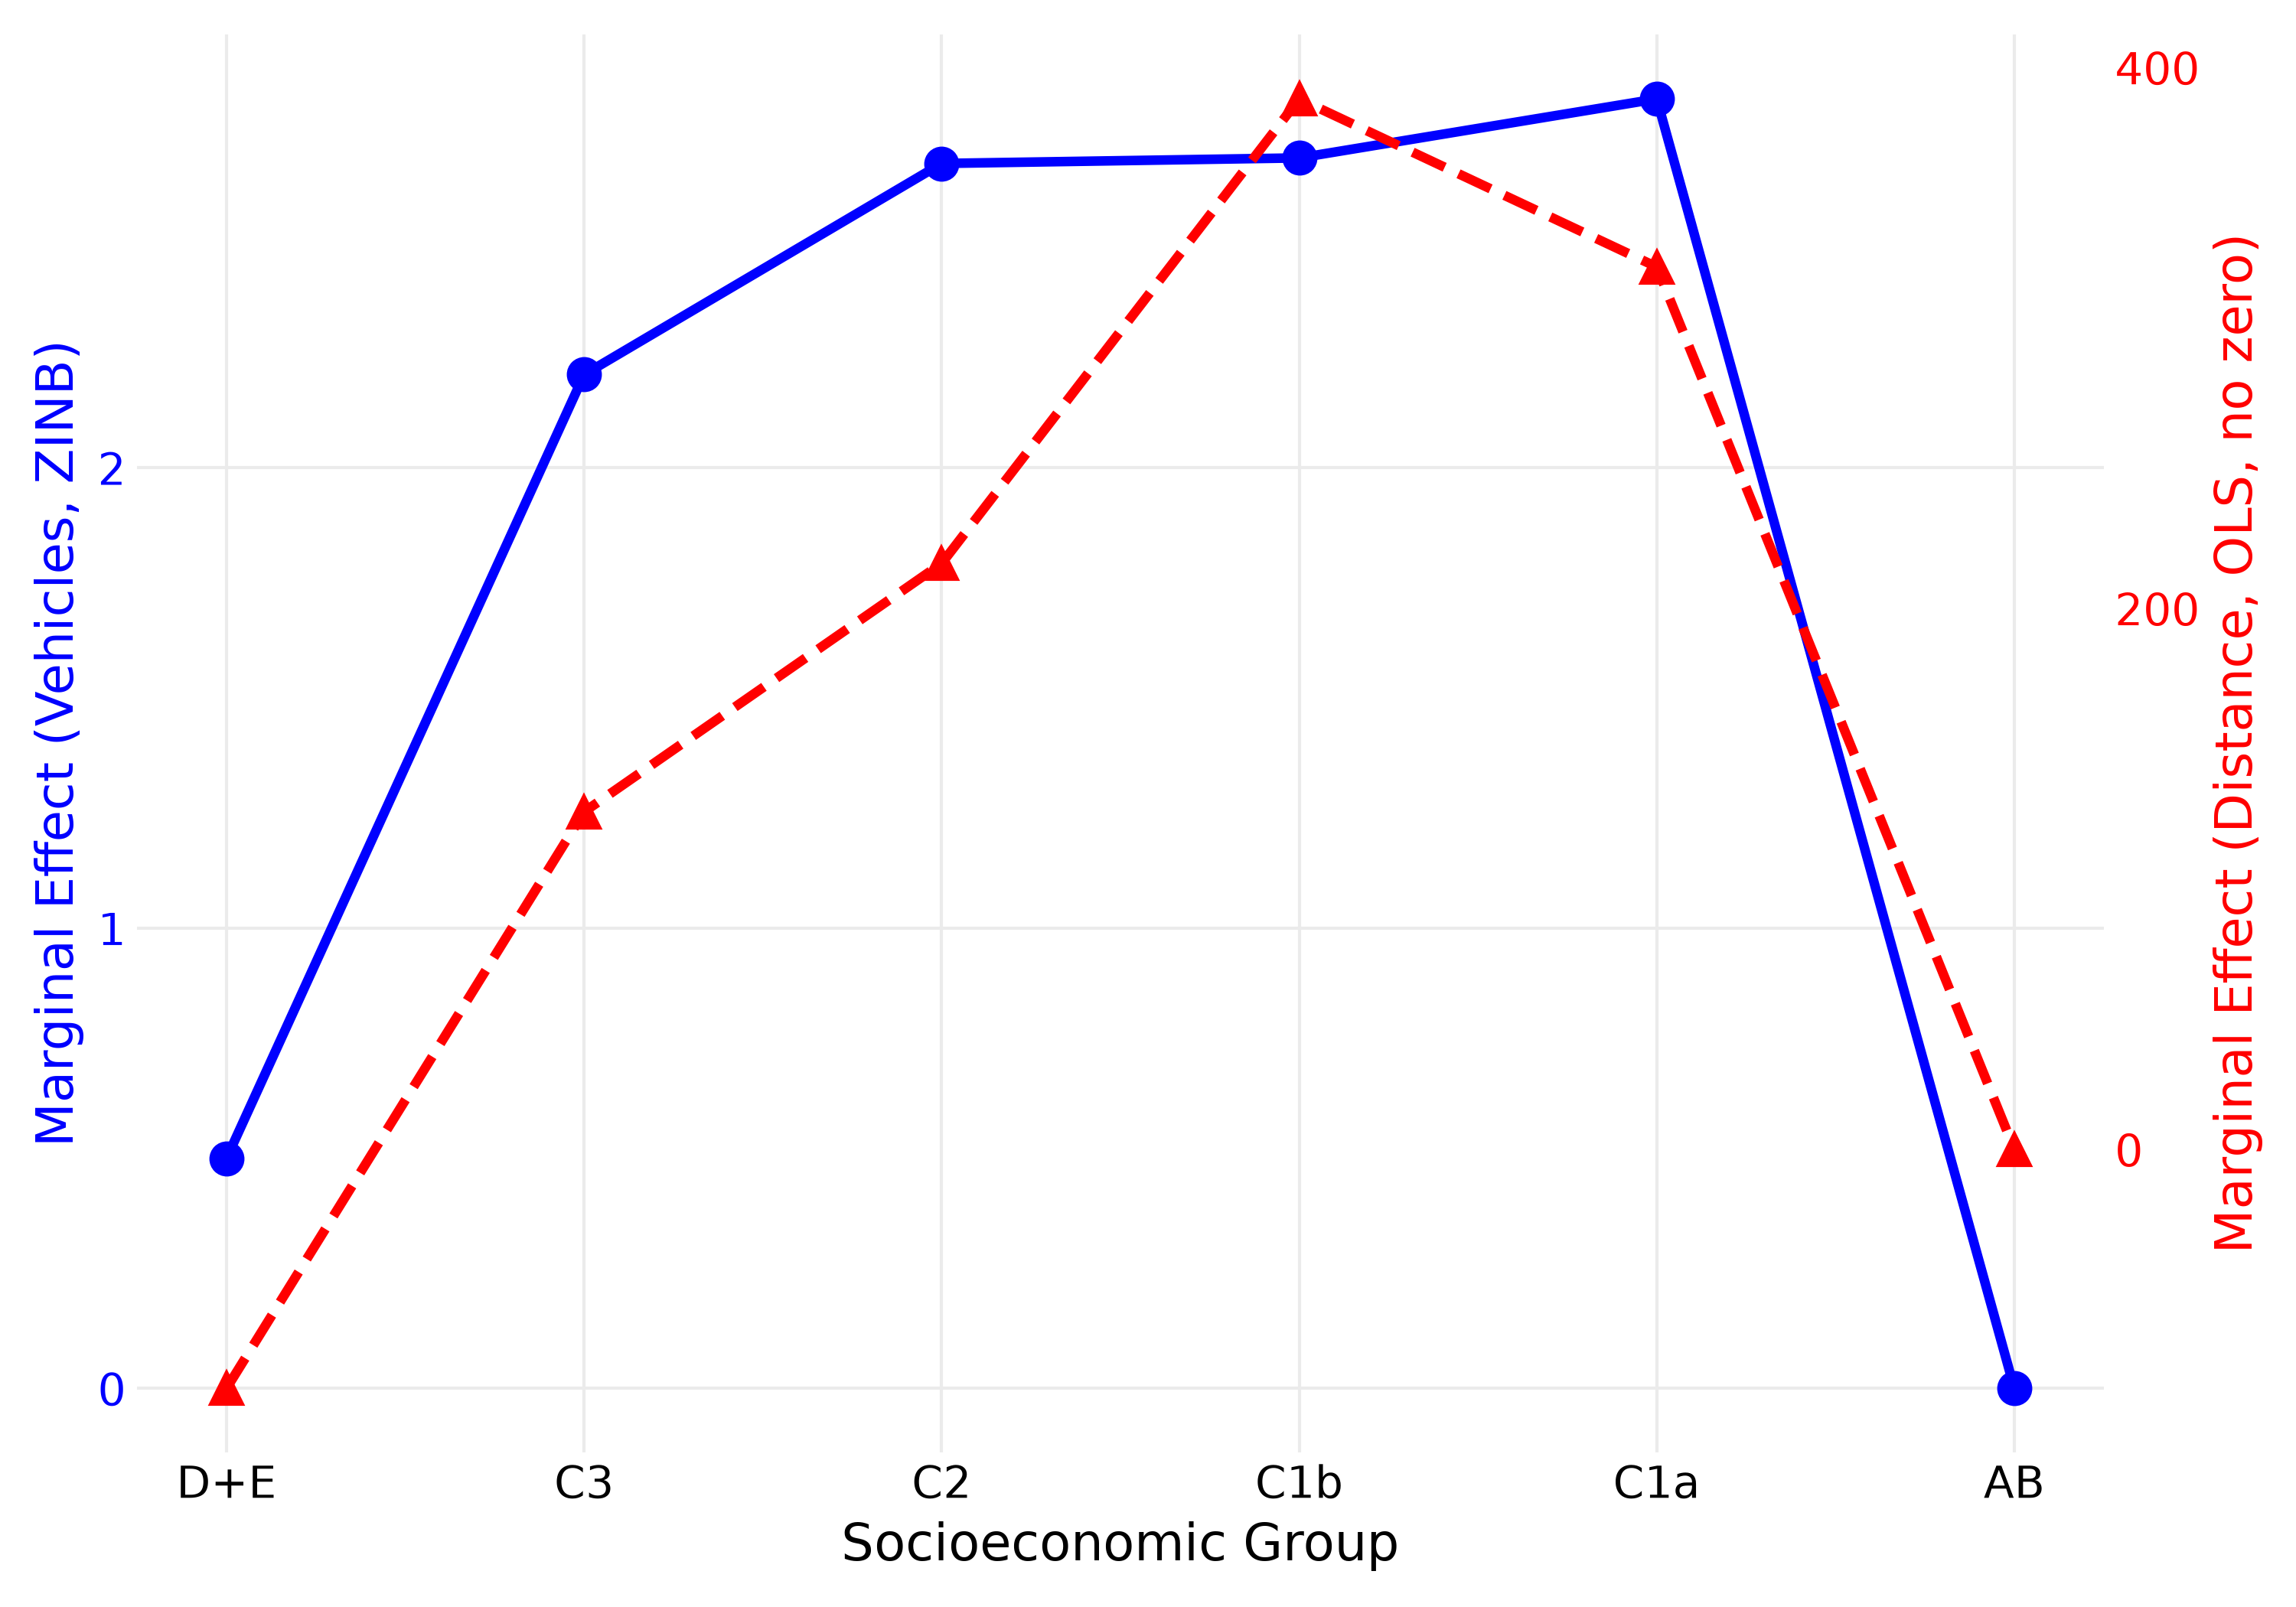
\includegraphics[width=\linewidth]{fig6_seg_dynamic.png}
%   \caption{Efectos marginales por grupo socioecon\'omico (modelo din\'amico).}
% \end{figure}

\printbibliography
\end{document}
